\section{Tercer captura: Red local muy chica}

\par Se realizó una tercer captura en una red local que poseía solamente tres hosts. La captura duró aproximadamente veinte minutos. En este caso vamos a analizar ambas fuentes de información.
\par En este experimento se tuvo una red con tres hosts, uno es el router (\textbf{192.168.1.1}), otro es dónde se estaba ejecutando la herramienta de monitoreo (\textbf{192.168.1.124}) mientras que en el equipo restante se estuvo realizando una descarga mediante un cliente torrent durante casi todo el tiempo (\textbf{192.168.1.129}).

\subsection{Resultados y análisis}

\par En el gráfico de barras en el que se compara la información de cada símbolo la fuente S con la entropía de la misma (figura 8) se puede ver que, al igual que en los demás experimentos hubo muchísimos más paquetes \textit{Broadcast} que \textit{Unicast}. Aún así el valor de la entropía está bastante cerca de ser el máximo, el cual es 0.5 ya que son dos símbolos.

\begin{figure}[h]
  \begin{subfigure}{.5\textwidth}
    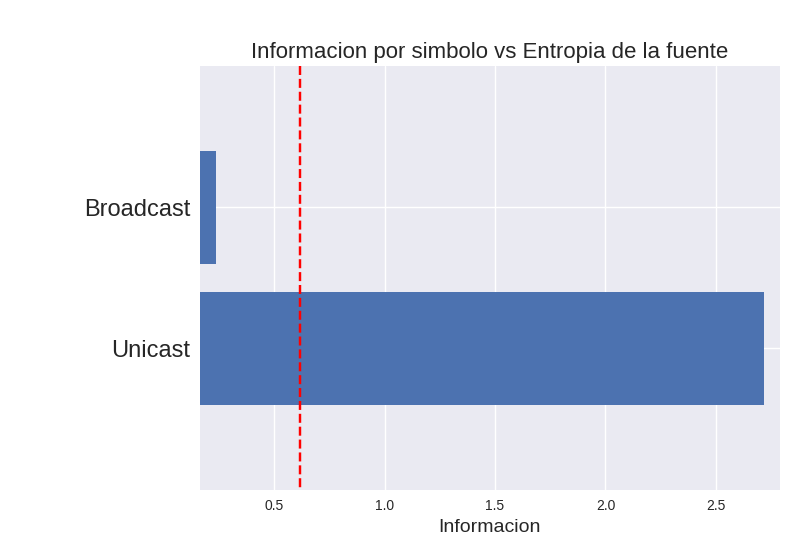
\includegraphics[width=\textwidth]{imagenes/mini_red/mini_red_unicastvsbroadcast.png}
  \end{subfigure}
  \label{fig:exp3_univsbr_infovsentro}
  \caption{Información de cada símbolo (Broadcast / Unicast) comparada con el valor de la entropía de la fuente de información (red local).}
\end{figure}

\par Con respecto al gráfico de barra de los hosts (figura 9), el equipo en el que se estuvo realizando la descarga tuvo una información muy baja y fue el único que estuvo por debajo de la entropía. Este resultado muestra una diferencia con las demás redes ya que el default gateway no resultó ser el de mayor probabilidad. Pero, es importante comentar que el host en el que se estaba iniciando una descarga envió paquetes ARP consultando por todas las direcciones posibles de la red. Por simplicidad del grafo no los incluimos a todas las direcciones de la red. También, en el grafo se puede ver una fuerte relación entre el host de la herramienta de monitoreo con el router como así también la de éste último con el equipo donde se estaba realizando la descarga.

\begin{figure}[h]
  \begin{subfigure}{.5\textwidth}
    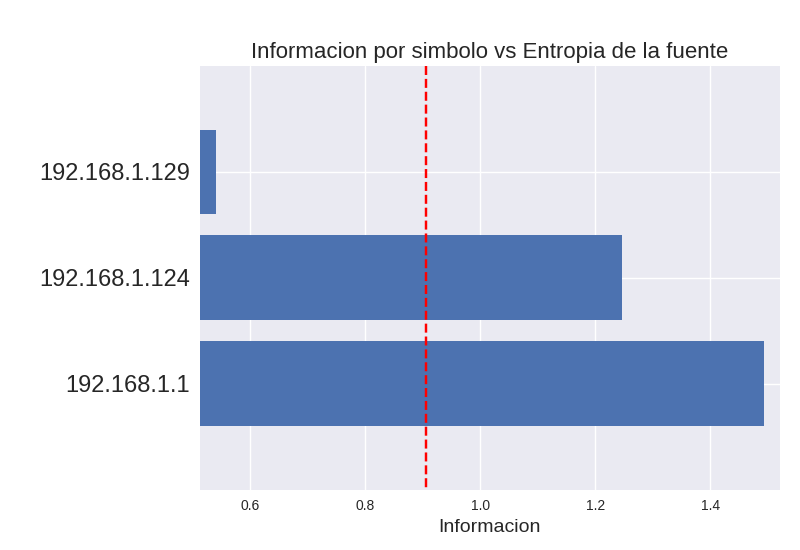
\includegraphics[width=\textwidth]{imagenes/mini_red/mini_red_hosts.png}
  \end{subfigure}
  \label{fig:exp3_hosts_infovsentro}
  \caption{Información de cada símbolo (host) comparada con el valor de la entropía de la fuente de información (red local).}
\end{figure}

\subsection{Conclusiones}

\par La entropía máxima es 0.5 ya que son 2 símbolos pero en este caso no se logró llegar a dicho valor. Esto sugiere que hay muchos envíos de mensajes de control, secuencia, etc. ya que éstos suelen ser broadcast. Este resultado está muy relacionado con el overhead de la red ya que los mensajes de control ocupan ancho de banda que, en algún caso, podrían enviarse datos.

\begin{figure}[h]
  \begin{subfigure}{.5\textwidth}
    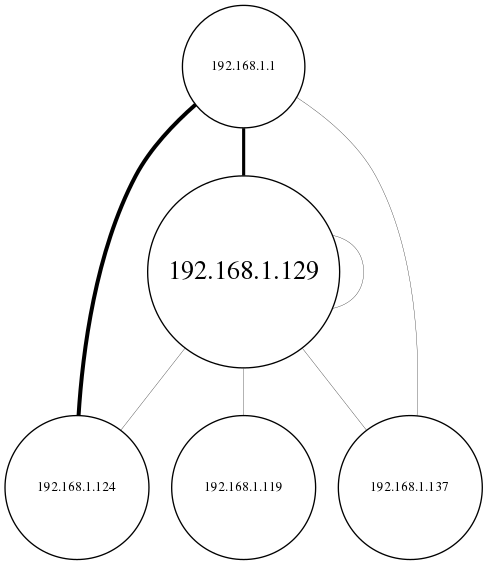
\includegraphics[width=\textwidth]{imagenes/mini_red/mini_red_Red.png}
  \end{subfigure}
  \label{fig:exp3_red}
  \caption{Diagrama de cómo creemos que está organizada la red de la tercer captura.}
\end{figure}

\par En esta red se puede distinguir solamente un nodo (\textbf{192.168.1.129}) pero fue un comportamiento por demás anómalo, por lo que no le podemos asignar ninguna función en especial dentro de la red. Creemos que si la captura hubiera durado alrededor de dos horas, el router (\textbf{192.168.124.1}) hubiera tenido mucha más participación. En particular por ser una red muy pequeña es esperable que se distinga un nodo, aunque si es inesperado qué nodo resultó ser.

\par Lamentablemente no hay una correspondencia entre lo que se conoce de la red y el resultado del experimento ya que la captura no duró lo suficiente y este outlier no nos permitió dilucidar la identidad de la puerta de enlace predeterminada.


\section{Cuarta captura: red intermedia}

\par En este último experimento, ejecutamos nuestro sniffer en una casa de comidas rápidas muy concurrida. La red es más grande que una hogareña pero más pequeña que la presentada en el primer experimento. La captura duró aproximadamente media hora.

\subsection{Resultados y análisis}

\par Como esta red posee muchísimos nodos decidimos realizar el gráfico con los que tienen menor información, en el mismo (figura 11) se pueden ver que hay algunos hosts con menos información que la entropía, mientras que hay otros que no. Pero en realidad todo los hosts restantes, es decir los que no fueron incluidos en el gráfico, tienen una información mayor. El host de la ip terminada en 110 es la puerta de enlace predeterminada, por lo cual es lógico que tenga mucha interacción con otros hosts. En la red hubo en total 127 hosts.

\begin{figure}[h]
  \begin{subfigure}{.5\textwidth}
    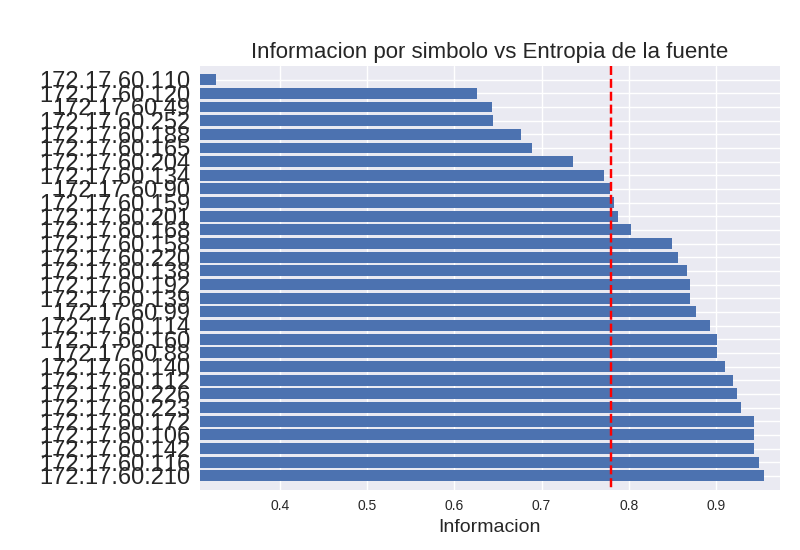
\includegraphics[width=\textwidth]{imagenes/mc/mchosts.png}
  \end{subfigure}
  \label{fig:exp4_hosts_infovsentro}
  \caption{Información de cada símbolo (host) comparada con el valor de la entropía de la fuente de información (red local).}
\end{figure}

\begin{figure*}[ht]
  \hspace*{-0.5cm}
  \begin{subfigure}{1.1\textwidth}
    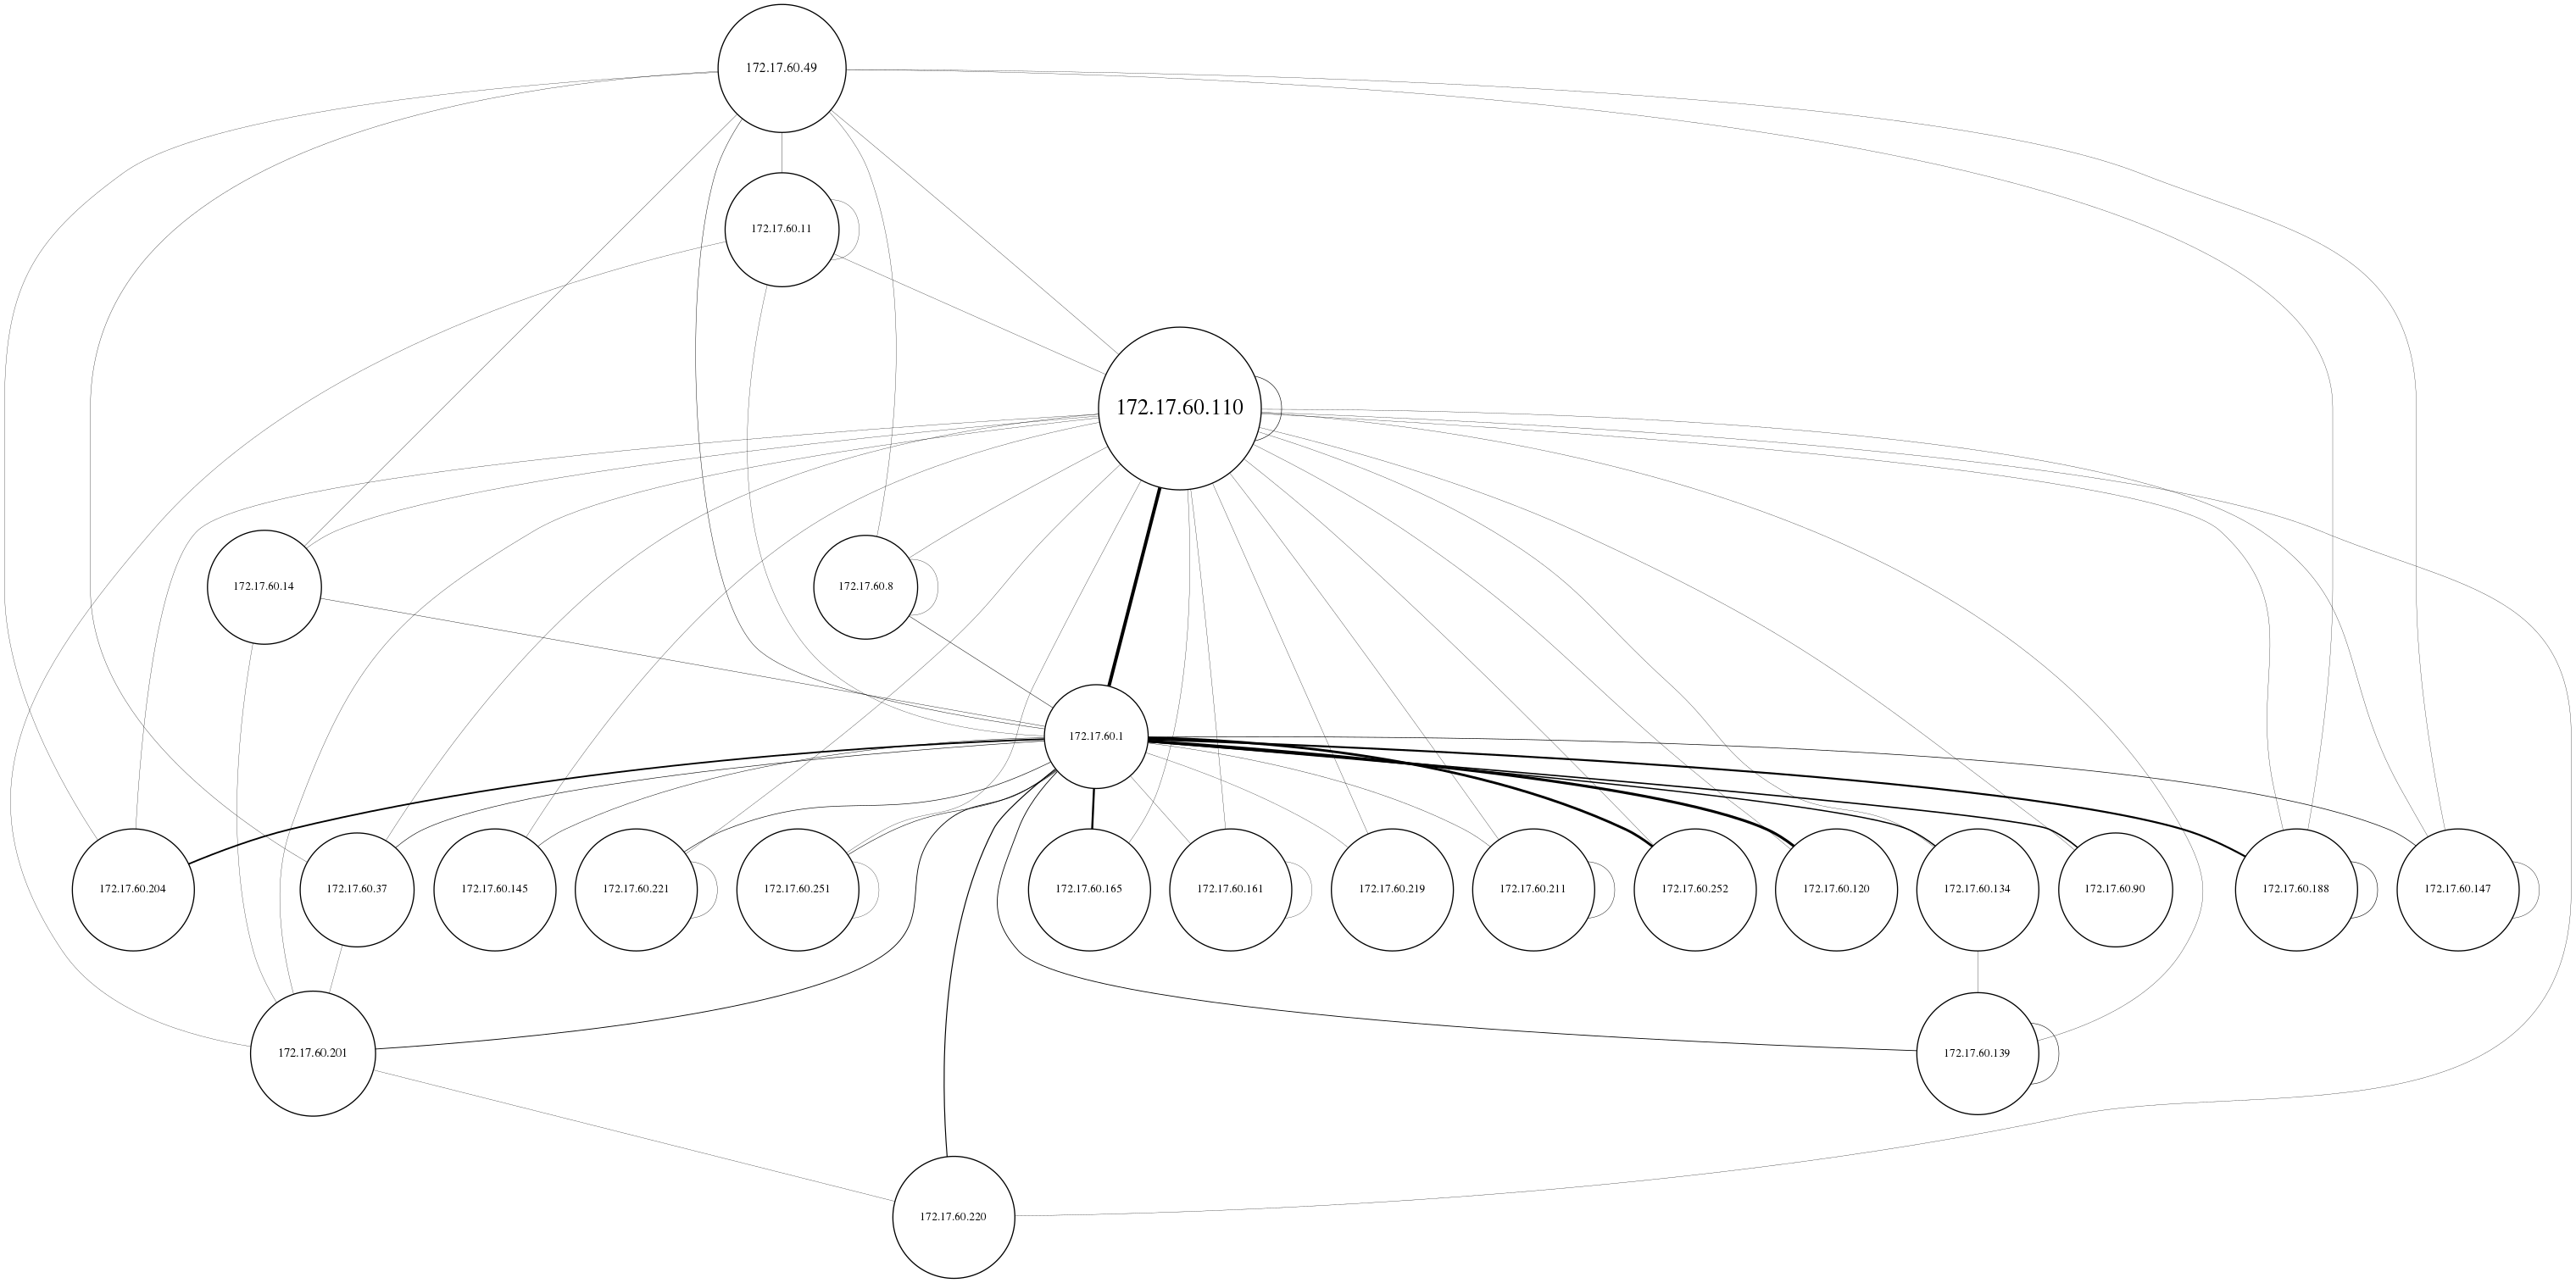
\includegraphics[width=\textwidth]{imagenes/mc/mcRed.png}
  \end{subfigure}
	\label{fig:exp4_grafo}
	\caption{Diagrama de cómo creemos que está organizada la red de la cuarta captura.}
\end{figure*}

\par Por otra parte, en el gráfico de barras en el que se compara la información de los paquetes \textit{Broadcast} contra la de los paquetes \textit{Unicast} (figura 12) se puede ver que hubo una gran diferencia a favor de la cantidad de paquetes broadcast en cuanto a paquetes enviados. Esto es sumamente razonable ya que la gran mayoría de los dispositivos conectados a la red son clientes.

\begin{figure}[h]
  \begin{subfigure}{.5\textwidth}
    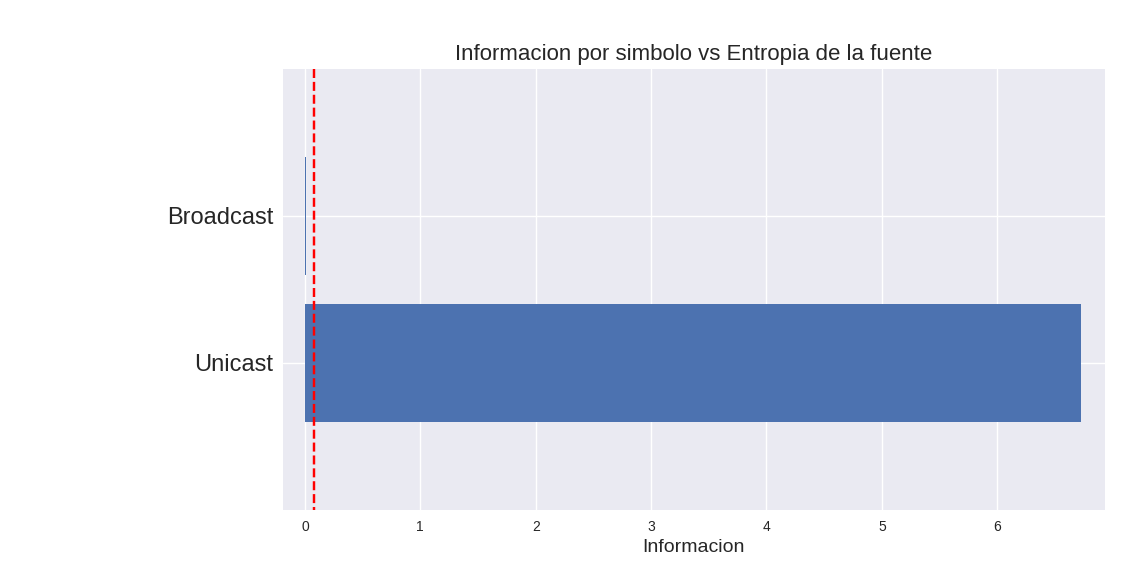
\includegraphics[width=\textwidth]{imagenes/mc/mcbrvsuni.png}
  \end{subfigure}
  \label{fig:exp4_univsbr_infovsentro}
  \caption{Información de cada símbolo (Broadcast / Unicast) comparada con el valor de la entropía de la fuente de información (red local).}
\end{figure}

\par Con respecto al grafo en el que mostramos los nodos distinguidos, podemos ver que el nodo \textbf{172.17.60.110} tiene muchísima más participación que el resto de los nodos. En particular, notamos que preguntó aproximadamente una vez por cada nodo pero, en cambio, sólo recibió preguntas de él mismo y del host \textbf{172.17.60.49}. Además, el nodo correspondiente al equipo cuya IP es \textbf{172.17.60.1} suele ser muy solicitado por la gran mayoría de los equipos de la red, pero en contrapartida éste no consultó en ningún momento por los demás.

\subsection{Conclusiones}
\par En este caso, la fuente S no tiene entropía máxima ya que hay muchos mensajes de control (por la gran cantidad de nodos activos que tiene la red). Además, por la longitud de la captura se acentuó esta tendencia, ya que muchos equipos no permanecieron durante toda la captura (recordemos que es un local de comida rápida). De esta manera hay mucho overhead en esta red.
\par En esta red se pudieron distinguir varios nodos (nueve en total). Son bastantes pocos con respecto al tamaño de la red pero, aún así, es razonable porque una red que tenga todos los nodos con un tráfico parejo no es conveniente. Pudimos notar que hubo un nodo que se comportó de manera no esperada, el nodo \textbf{172.17.60.1}. Este nodo hacía de intermediario entre la gran mayoría de los nodos de la red y el default gateway (\textbf{172.17.60.110}).
\par Gracias al resultado de la captura podemos afirmar que el default gateway es el equipo cuya ip es \textbf{172.17.60.110}. Nos convencemos también de que la herramienta también sirve para detectar puntos intermedios de paso hasta llegar al router.
